\chapter{Expected Results and Evaluation Plan}
\label{chap:ExpectedResults}

This chapter outlines the anticipated outcomes of the research and the comprehensive plan designed to evaluate the developed system. The expected results are presented across several dimensions: the system's technical architecture, its performance and quality benchmarks, its clinical impact, user acceptance, and financial viability. The evaluation plan details the methodology, metrics, and instruments that will be used to measure the success of the implementation in a live hospital environment.

\section{Proposed System Architecture}

The system's design will be guided by the principles of modularity, scalability, and maintainability, culminating in a layered microservices architecture. This architectural choice, illustrated in Figure~\ref{fig:architecture}, is considered critical for managing the complexity of the hospital environment and ensuring a clear separation of concerns. This approach will facilitate parallel development, independent deployment of services, and greater resilience compared to monolithic designs \cite{newman2015}.

\begin{figure}[htbp]
    \centering
    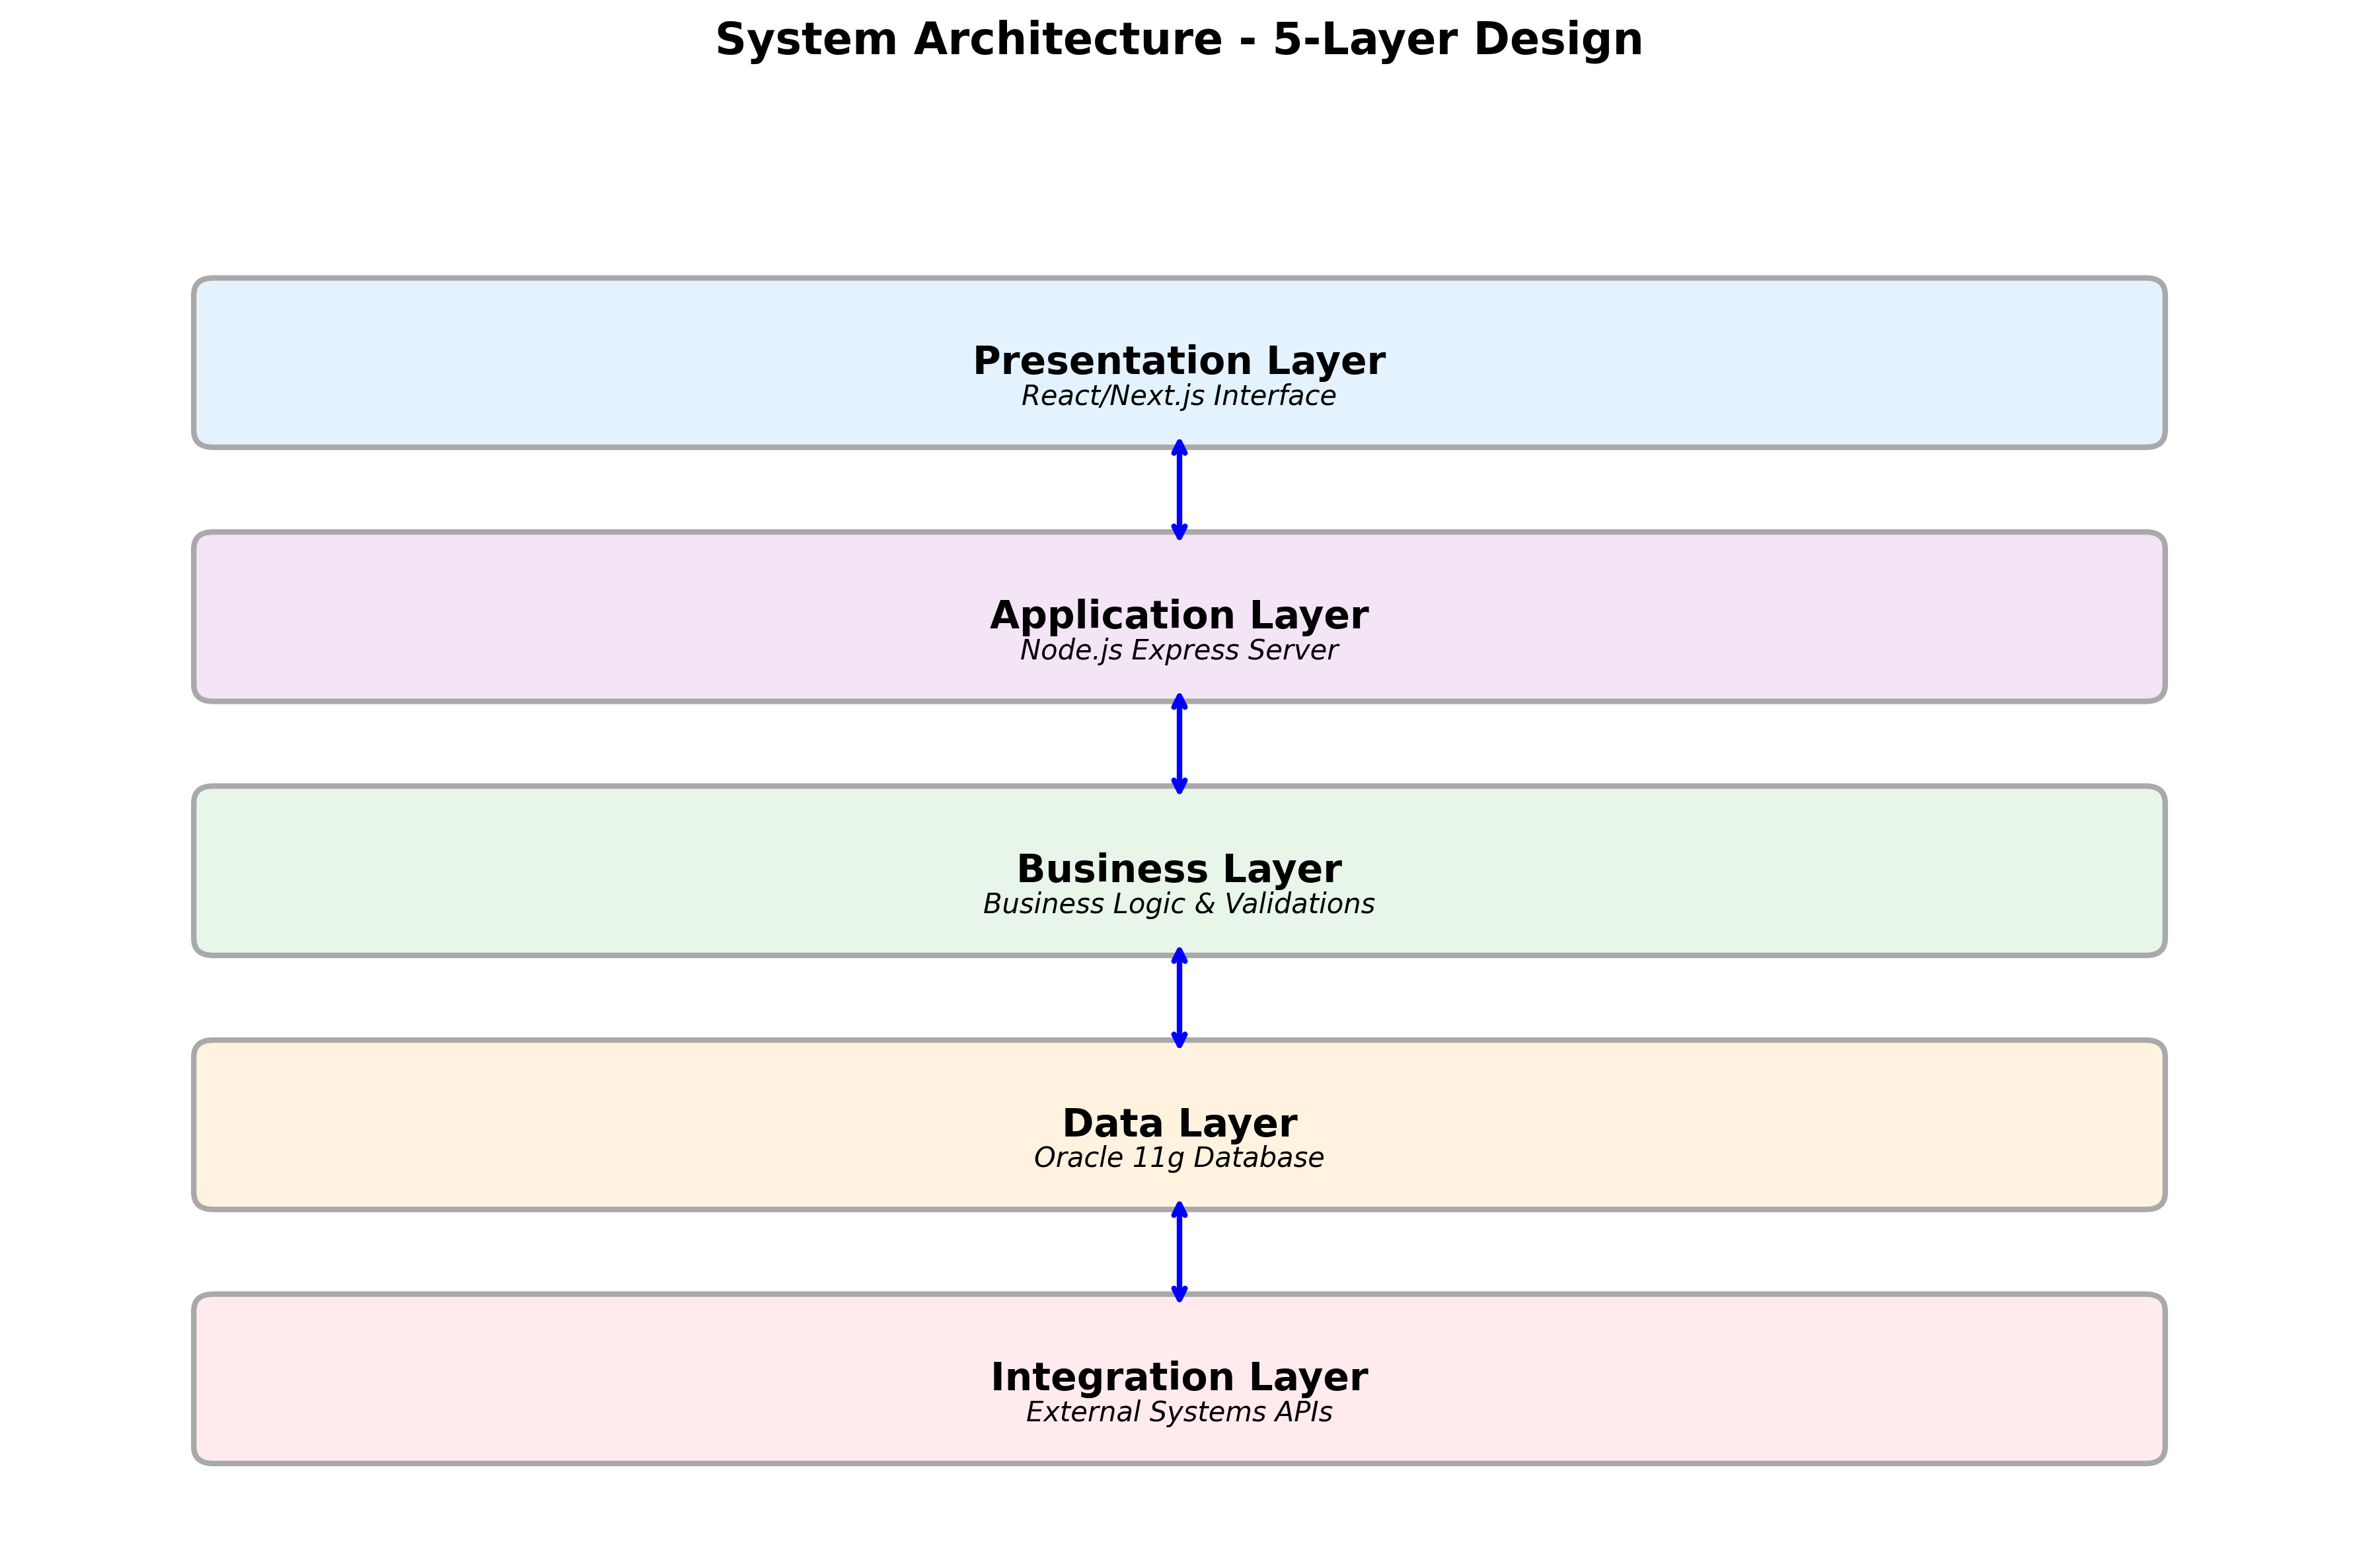
\includegraphics[width=0.95\textwidth]{images/generated/system_architecture.png}
    \caption{Layered architecture of the medication management system, detailing internal components and integrations with external systems.}
    \label{fig:architecture}
\end{figure}

The proposed architecture will be composed of five distinct layers. The \textit{Presentation Layer}, built with React and Next.js, will provide a responsive and intuitive \gls{ui}. It will communicate with the \textit{Application Layer} (Node.js/Express), which will orchestrate \glspl{api} requests. The core clinical intelligence will reside in the \textit{Business Logic Layer}. Data persistence will be handled by the \textit{Data Layer}, using an optimized Oracle 11g database, while the \textit{Integration Layer} will provide a secure RESTful API for communication with other hospital systems.

Key components to be implemented include a robust authentication system integrated with the hospital's LDAP for \gls{sso} and a granular role-based access control model. The e-prescription module will feature real-time clinical decision support (\gls{cdss}), aiming to significantly reduce prescribing errors by validating prescriptions against a knowledge base for potential \gls{ddi} and allergies, a strategy proven effective in multiple studies \cite{bates2014}. The pharmaceutical validation system will be designed to provide a complete and immutable audit trail, enhancing accountability.

\section{Performance and Quality Benchmarks}

Rigorous performance and quality assurance will be central to the development methodology. It is expected that targeted optimizations will yield substantial performance gains. For instance, a key objective is to reduce the response time of critical search components to under one second through techniques like server-side caching. The goal for average API response time for most read operations is approximately 200ms, a critical threshold for maintaining user engagement in fast-paced clinical settings \cite{nielsen2012}.

A primary technical objective is to achieve seamless integration with existing hospital systems. The target is a 100\% success rate for data exports to the billing system and a reduction of over 90\% in data synchronization errors with legacy systems. This will be achieved by implementing robust validation and transformation pipelines. Furthermore, a disciplined refactoring effort will aim to increase automated test coverage to over 80\% and ensure the frontend achieves full compliance with \gls{wcag} 2.1 Level AA.

\section{Evaluation Plan and Expected Clinical Impact}

The system will undergo a six-month pilot evaluation in a live clinical environment at SCMVV to assess its real-world impact. During this period, it is anticipated that the system will be adopted by over 150 healthcare professionals and used to process thousands of prescriptions and medication administrations. The platform's reliability will be a key performance indicator (KPI), with a target of 99.95\% uptime, even under peak loads \cite{nkenyereye2016}.

The most significant expected outcome is a transformative impact on patient safety. As illustrated by the goals in Figure~\ref{fig:error-reduction}, the project aims for a reduction of over 70\% in prescribing errors and over 85\% in validation errors. These targets are ambitious but consistent with benchmarks reported in large-scale studies on the effects of similar systems \cite{radley2013, bates2014}. The introduction of end-to-end traceability is expected to reduce the time required to investigate medication-related incidents by 90\%.

\begin{figure}[htbp]
    \centering
    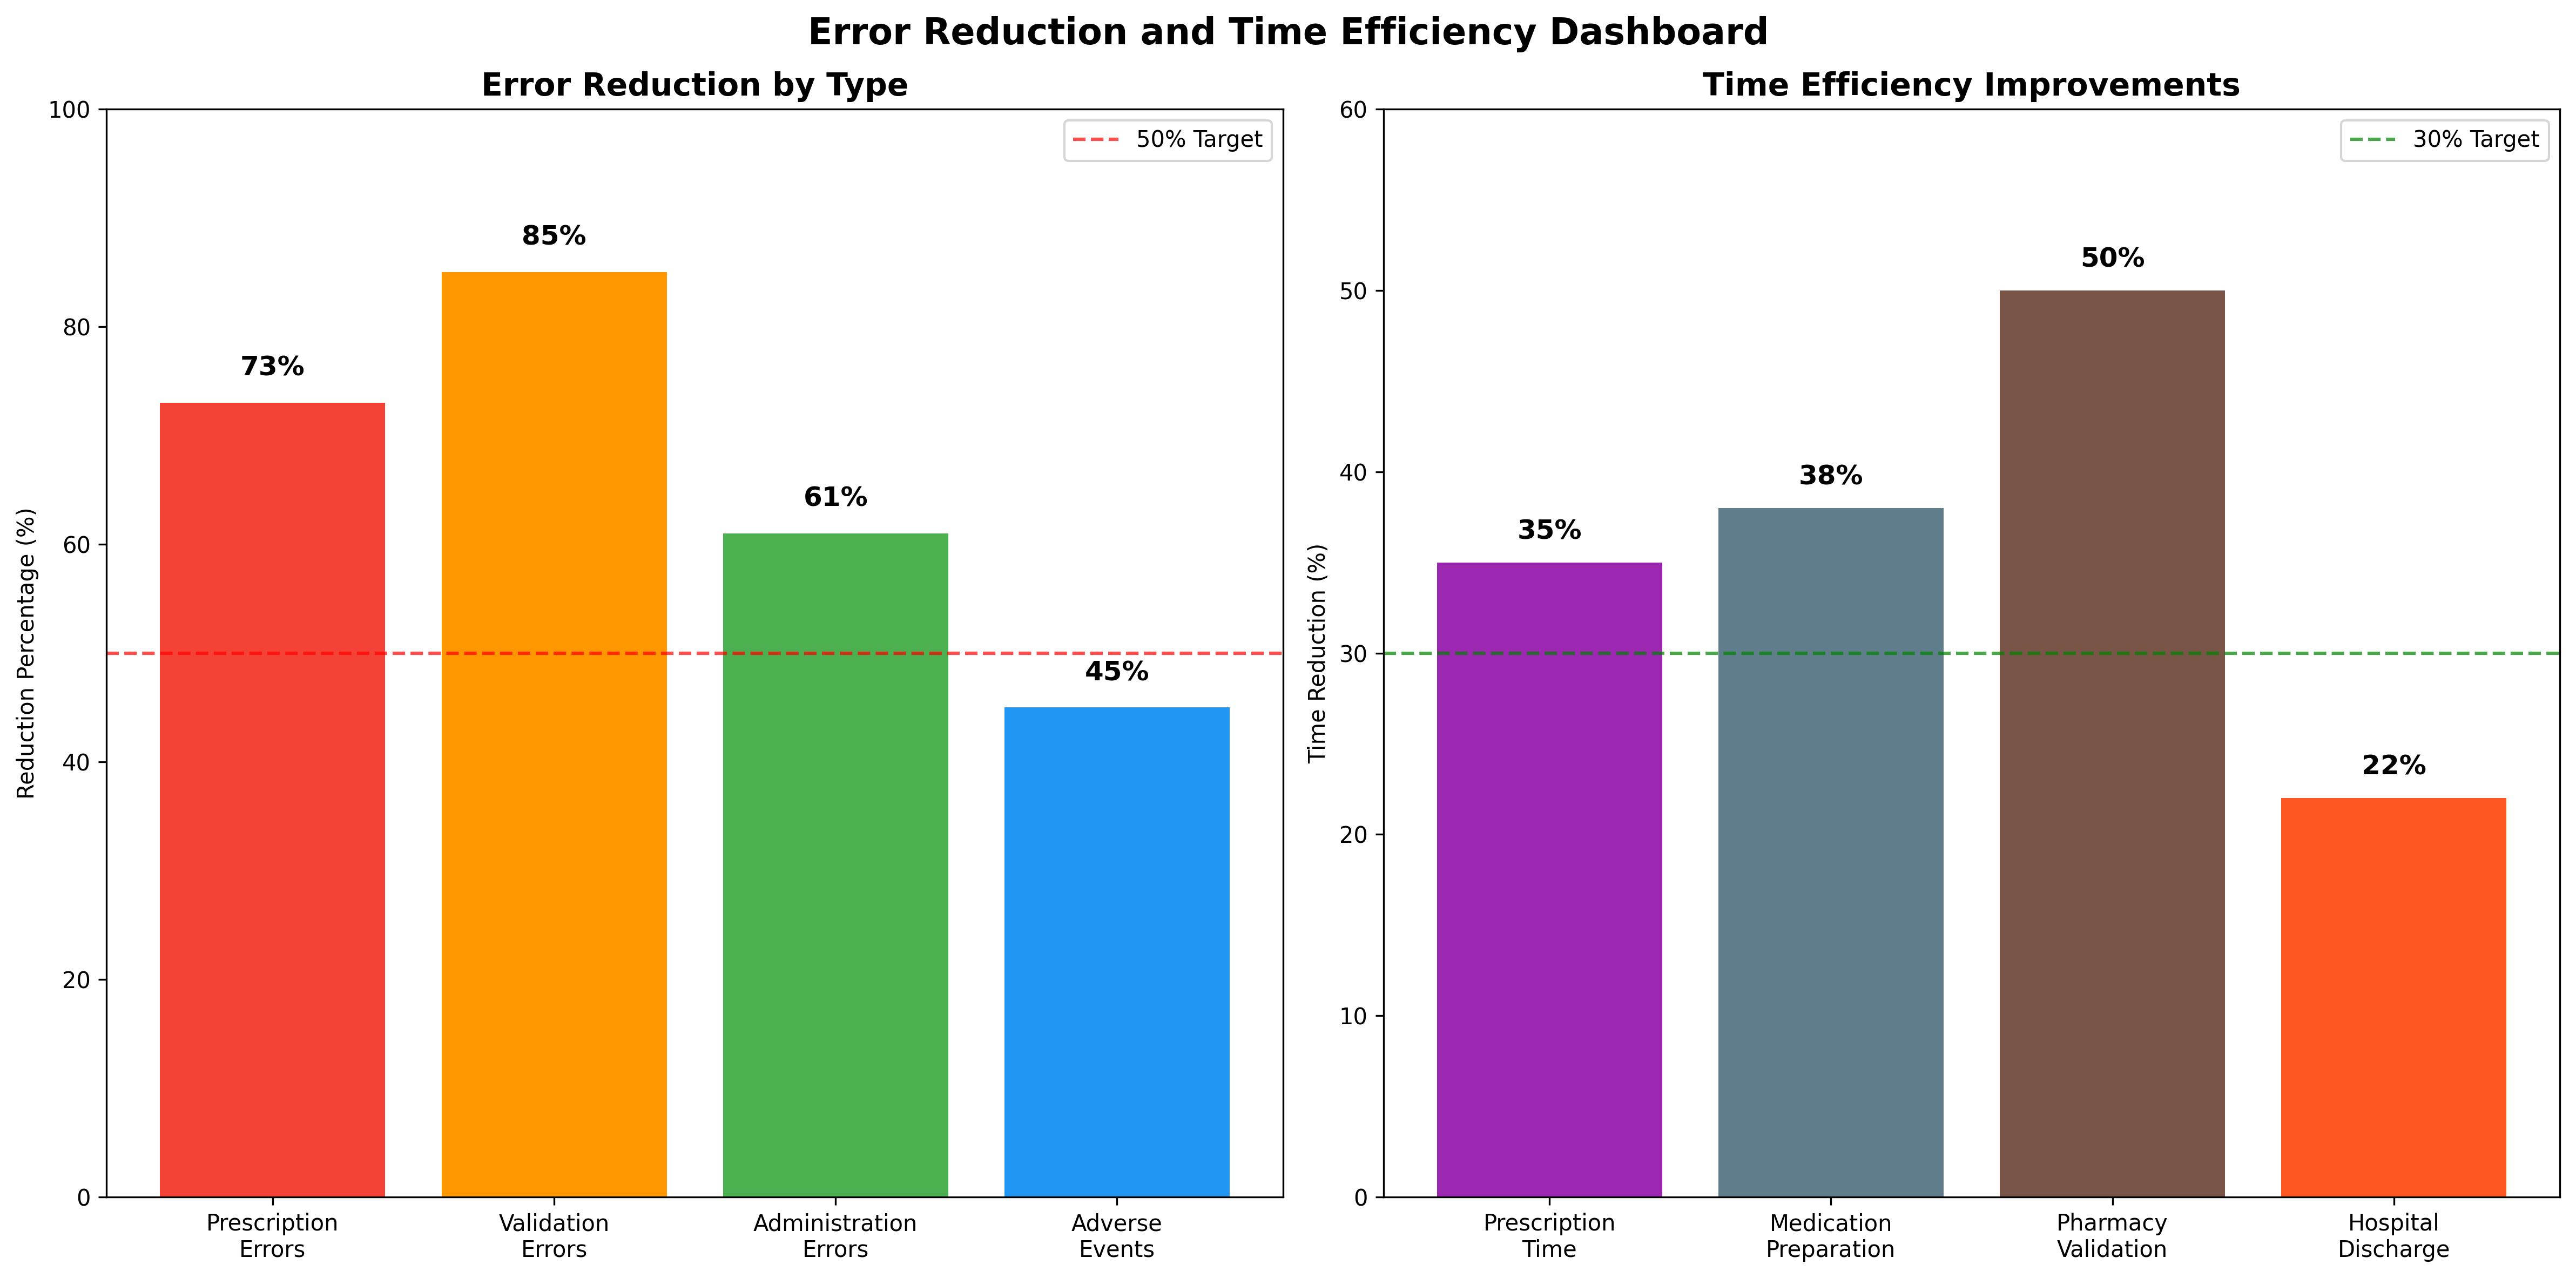
\includegraphics[width=0.95\textwidth]{images/generated/error_reduction_dashboard.png}
    \caption{Dashboard illustrating the reduction in medication errors and improvements in process efficiency following system implementation.}
    \label{fig:error-reduction}
\end{figure}

Significant gains in operational efficiency are also anticipated. The system is being designed to streamline clinical workflows, with the goal of reducing the time required for physicians to prescribe by at least 30\% and for pharmacists to validate by 40\%. This enhanced efficiency is expected to improve interdisciplinary communication, projecting an 80\% reduction in clarification requests from the pharmacy, thereby freeing up valuable clinical time for patient care \cite{austin2018}.

\section{User Acceptance Evaluation}

High user acceptance is critical for the success of this sociotechnical intervention. The evaluation of user acceptance will be conducted using the System Usability Scale (SUS), a standardized questionnaire. The target is to achieve a SUS score of 75 or higher, which would place the system in the "Good" to "Excellent" range and well above the average for healthcare IT systems \cite{lewis2018}. Achieving this score would validate the user-centered design approach.

Qualitative feedback will also be systematically collected through semi-structured interviews and focus groups with physicians, pharmacists, and nurses. As detailed in the evaluation plan (Figure~\ref{fig:user-satisfaction}), this feedback will be analyzed to assess confidence in the system, perceived safety improvements, and the clarity of workflows. A further metric will be the training time required for new users, with a goal of reducing it by over 60\% compared to the legacy system.

\begin{figure}[htbp]
    \centering
    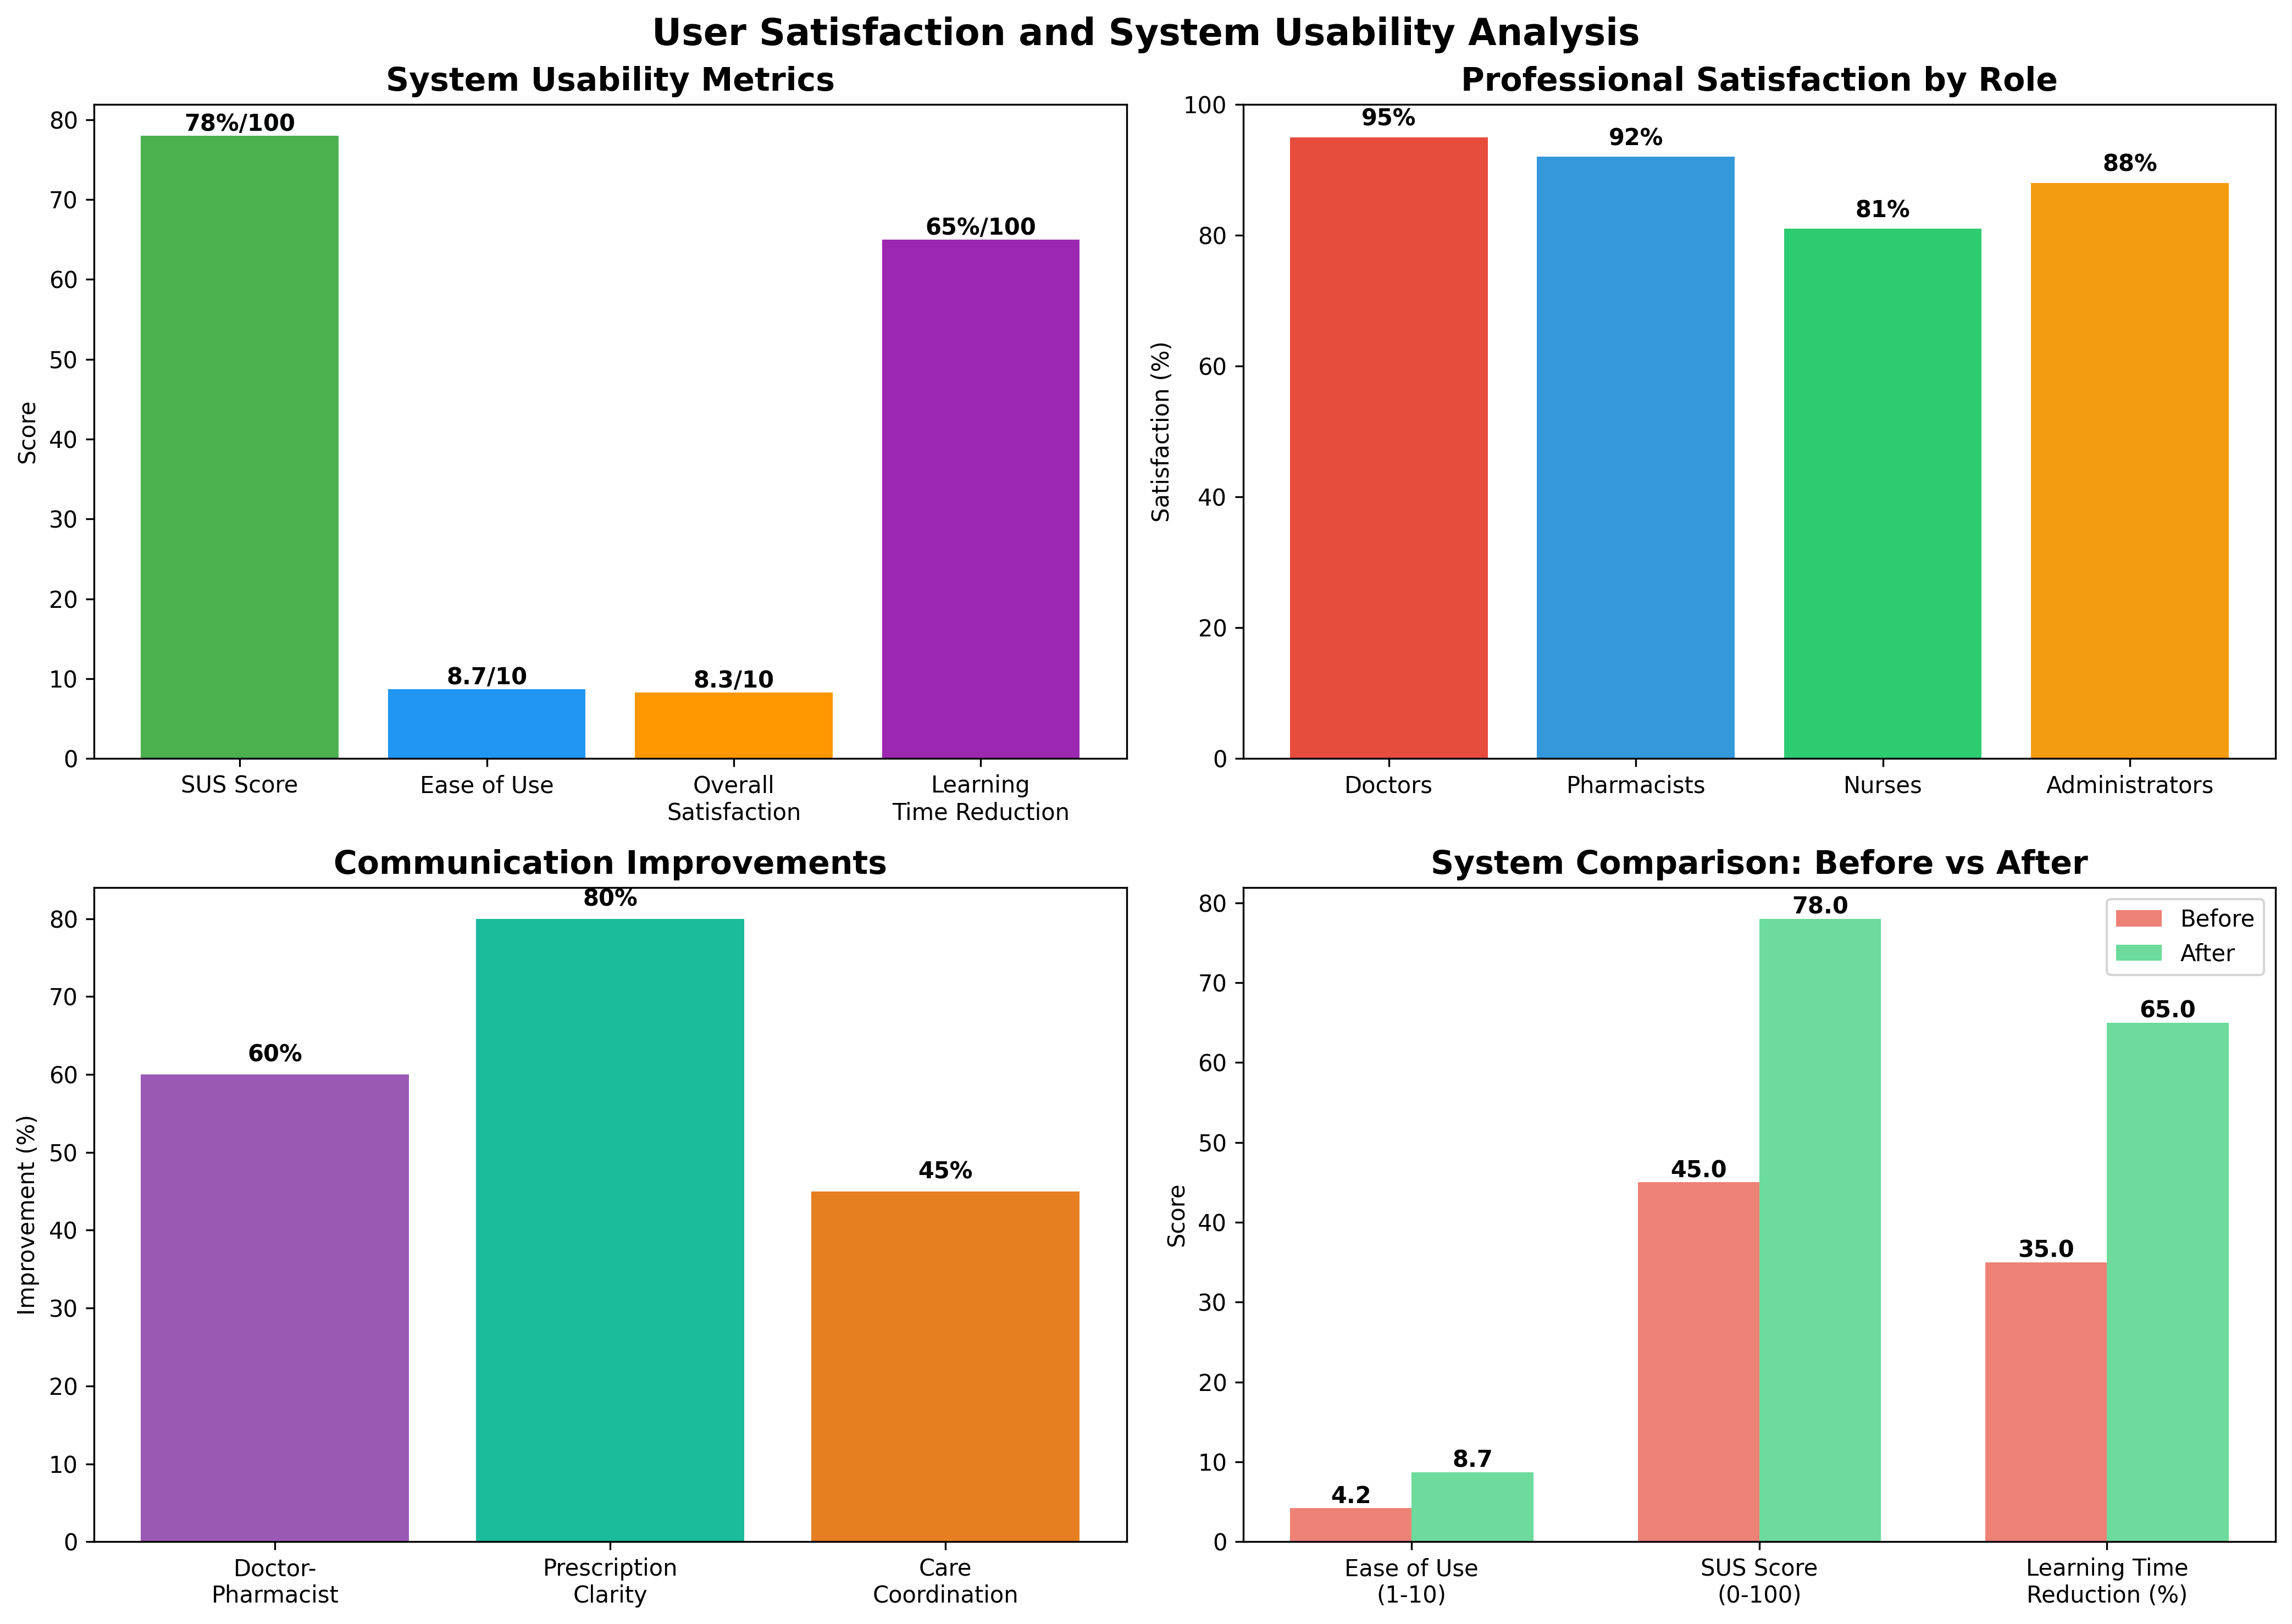
\includegraphics[width=0.95\textwidth]{images/generated/user_satisfaction.png}
    \caption{Comprehensive analysis of user satisfaction, including usability metrics, satisfaction ratings by professional category, and communication improvements.}
    \label{fig:user-satisfaction}
\end{figure}

\section{Expected Financial Impact and Future Viability}

A cost-benefit analysis will be conducted as part of the evaluation to determine the financial impact. Based on the expected efficiency gains and reduction in costs associated with medication errors, the analysis presented in Figure~\ref{fig:roi-analysis} projects a strong return on investment (ROI). The projected payback period is approximately 8 months, a figure that provides a compelling economic justification for the intervention when compared to industry averages \cite{adler2021}. This robust financial case, coupled with the system's planned scalability and the strategic roadmap (Figure~\ref{fig:future-roadmap}), is intended to ensure its long-term viability and potential for future expansion.

\begin{figure}[htbp]
    \centering
    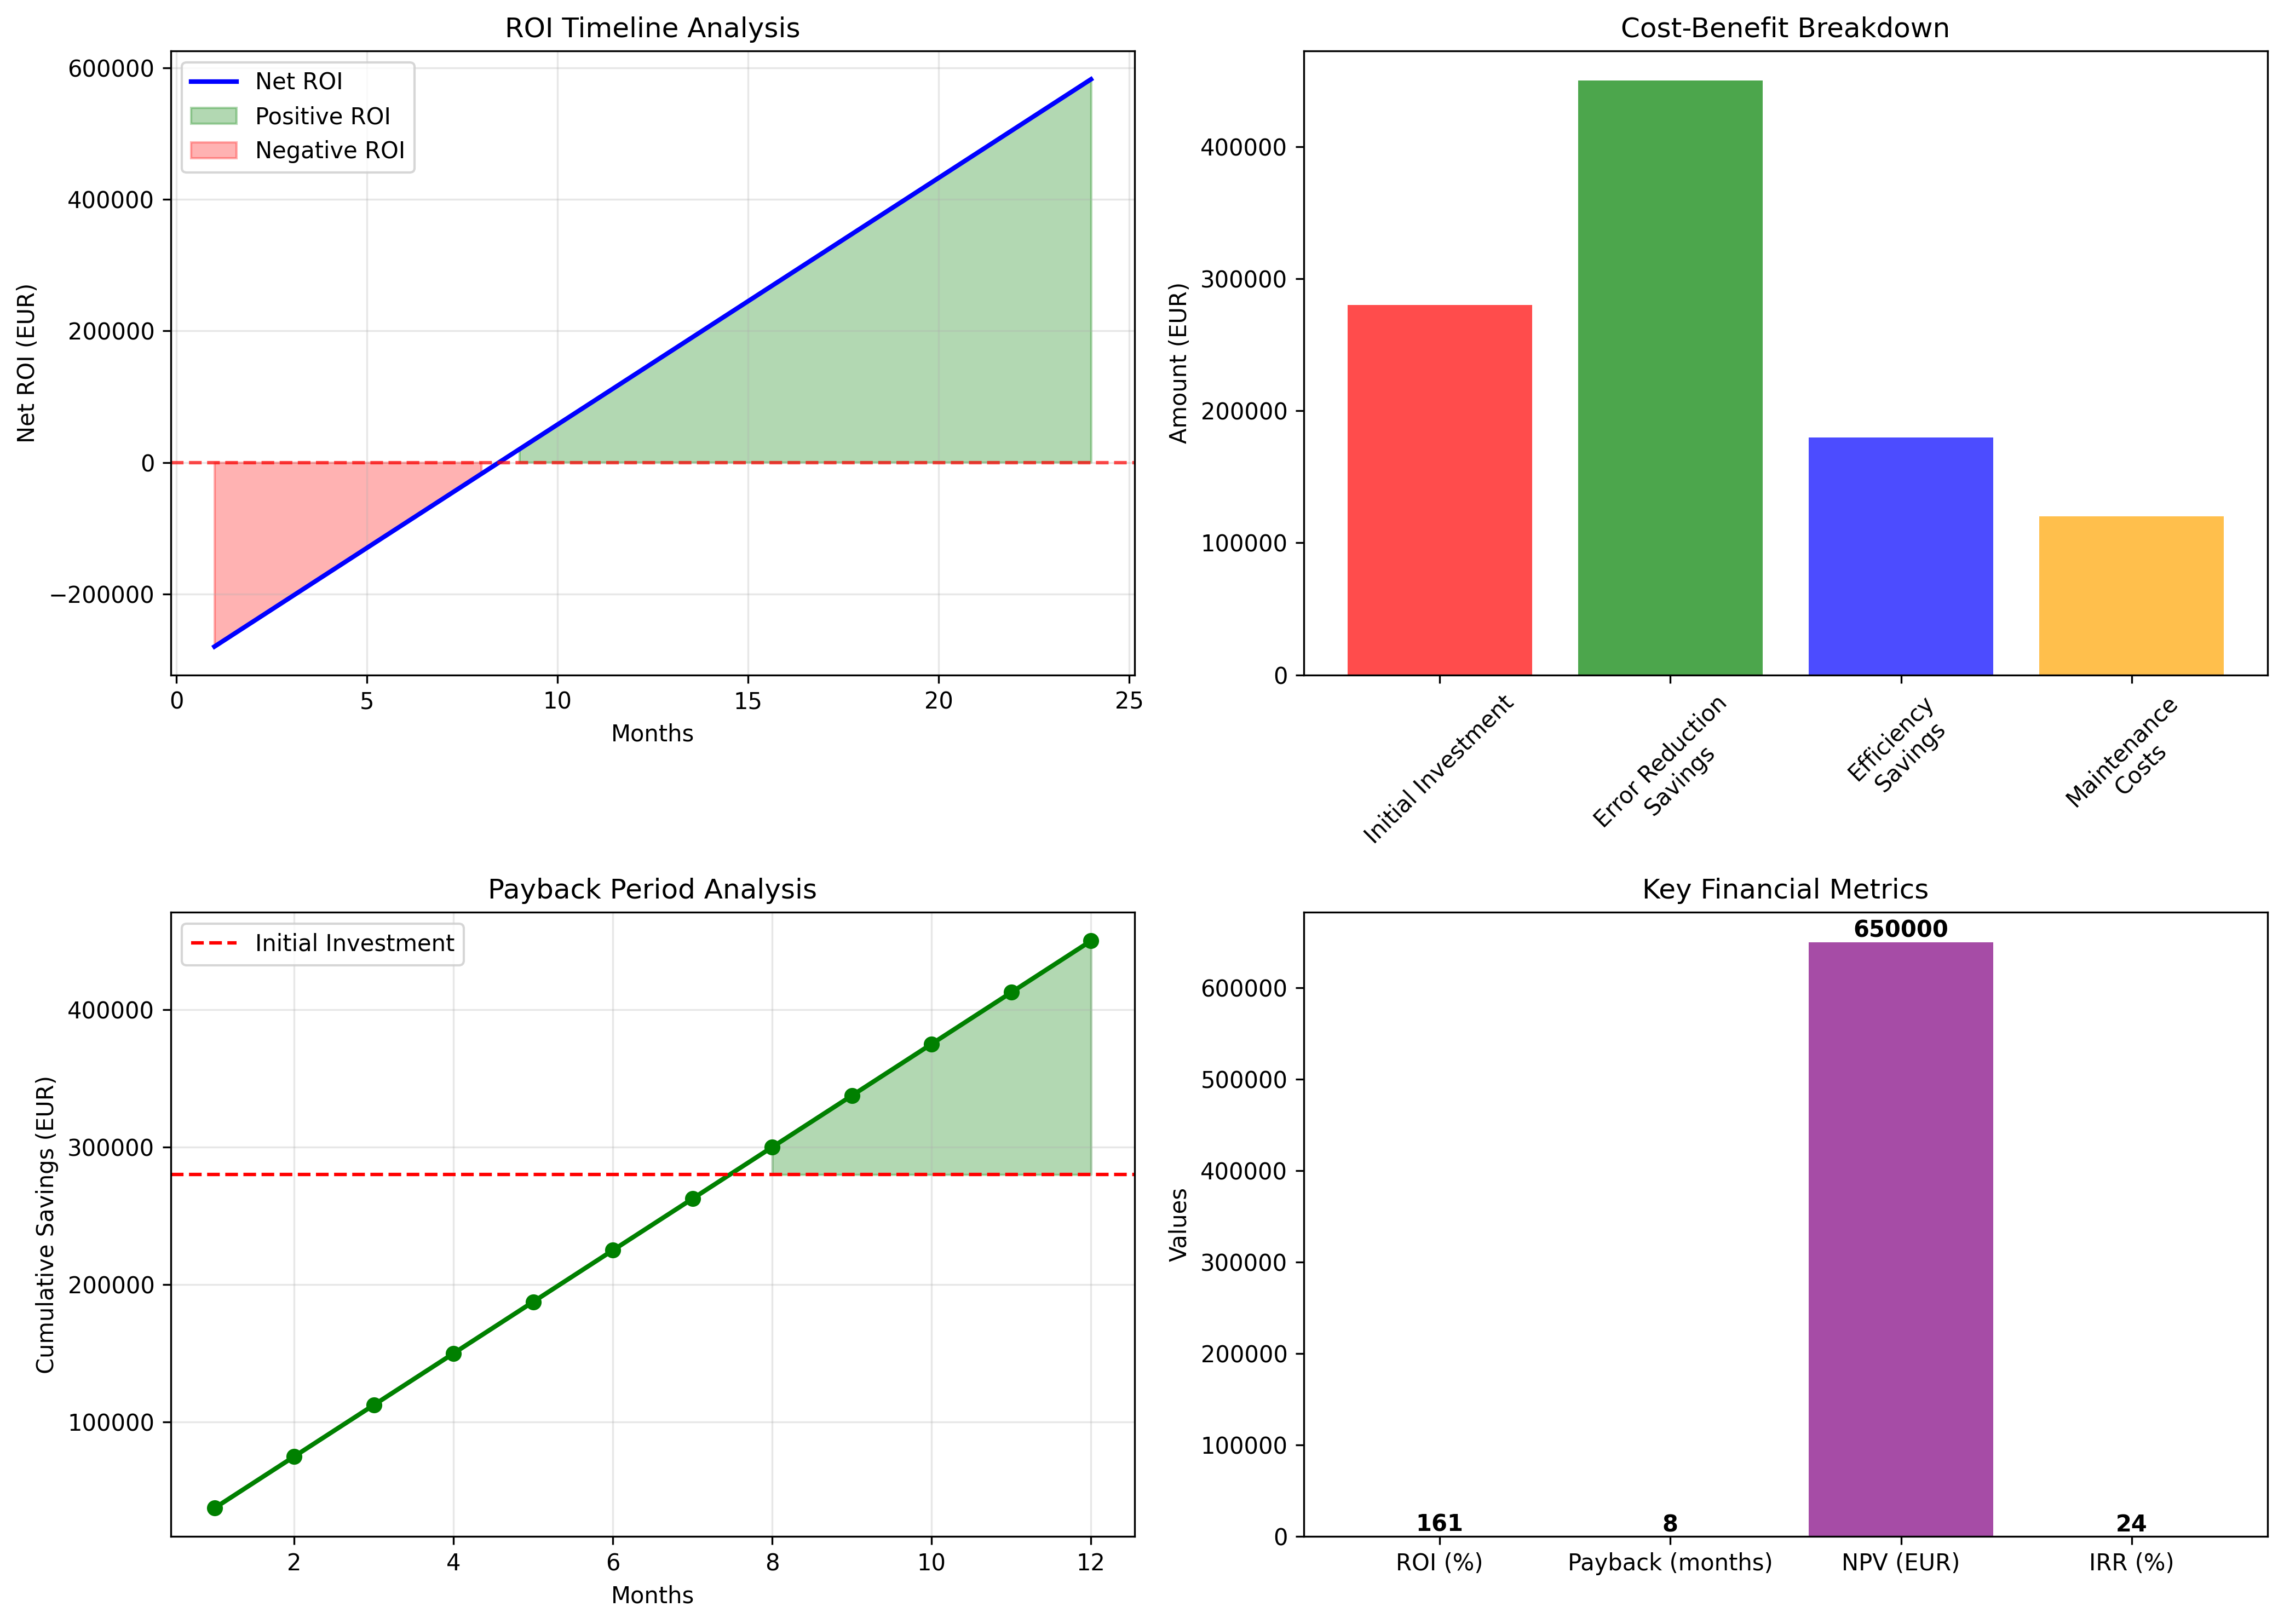
\includegraphics[width=0.95\textwidth]{images/generated/roi_analysis.png}
    \caption{Cost-benefit analysis, including investment breakdown, ROI timeline, and payback period calculation.}
    \label{fig:roi-analysis}
\end{figure}

\begin{figure}[htbp]
    \centering
    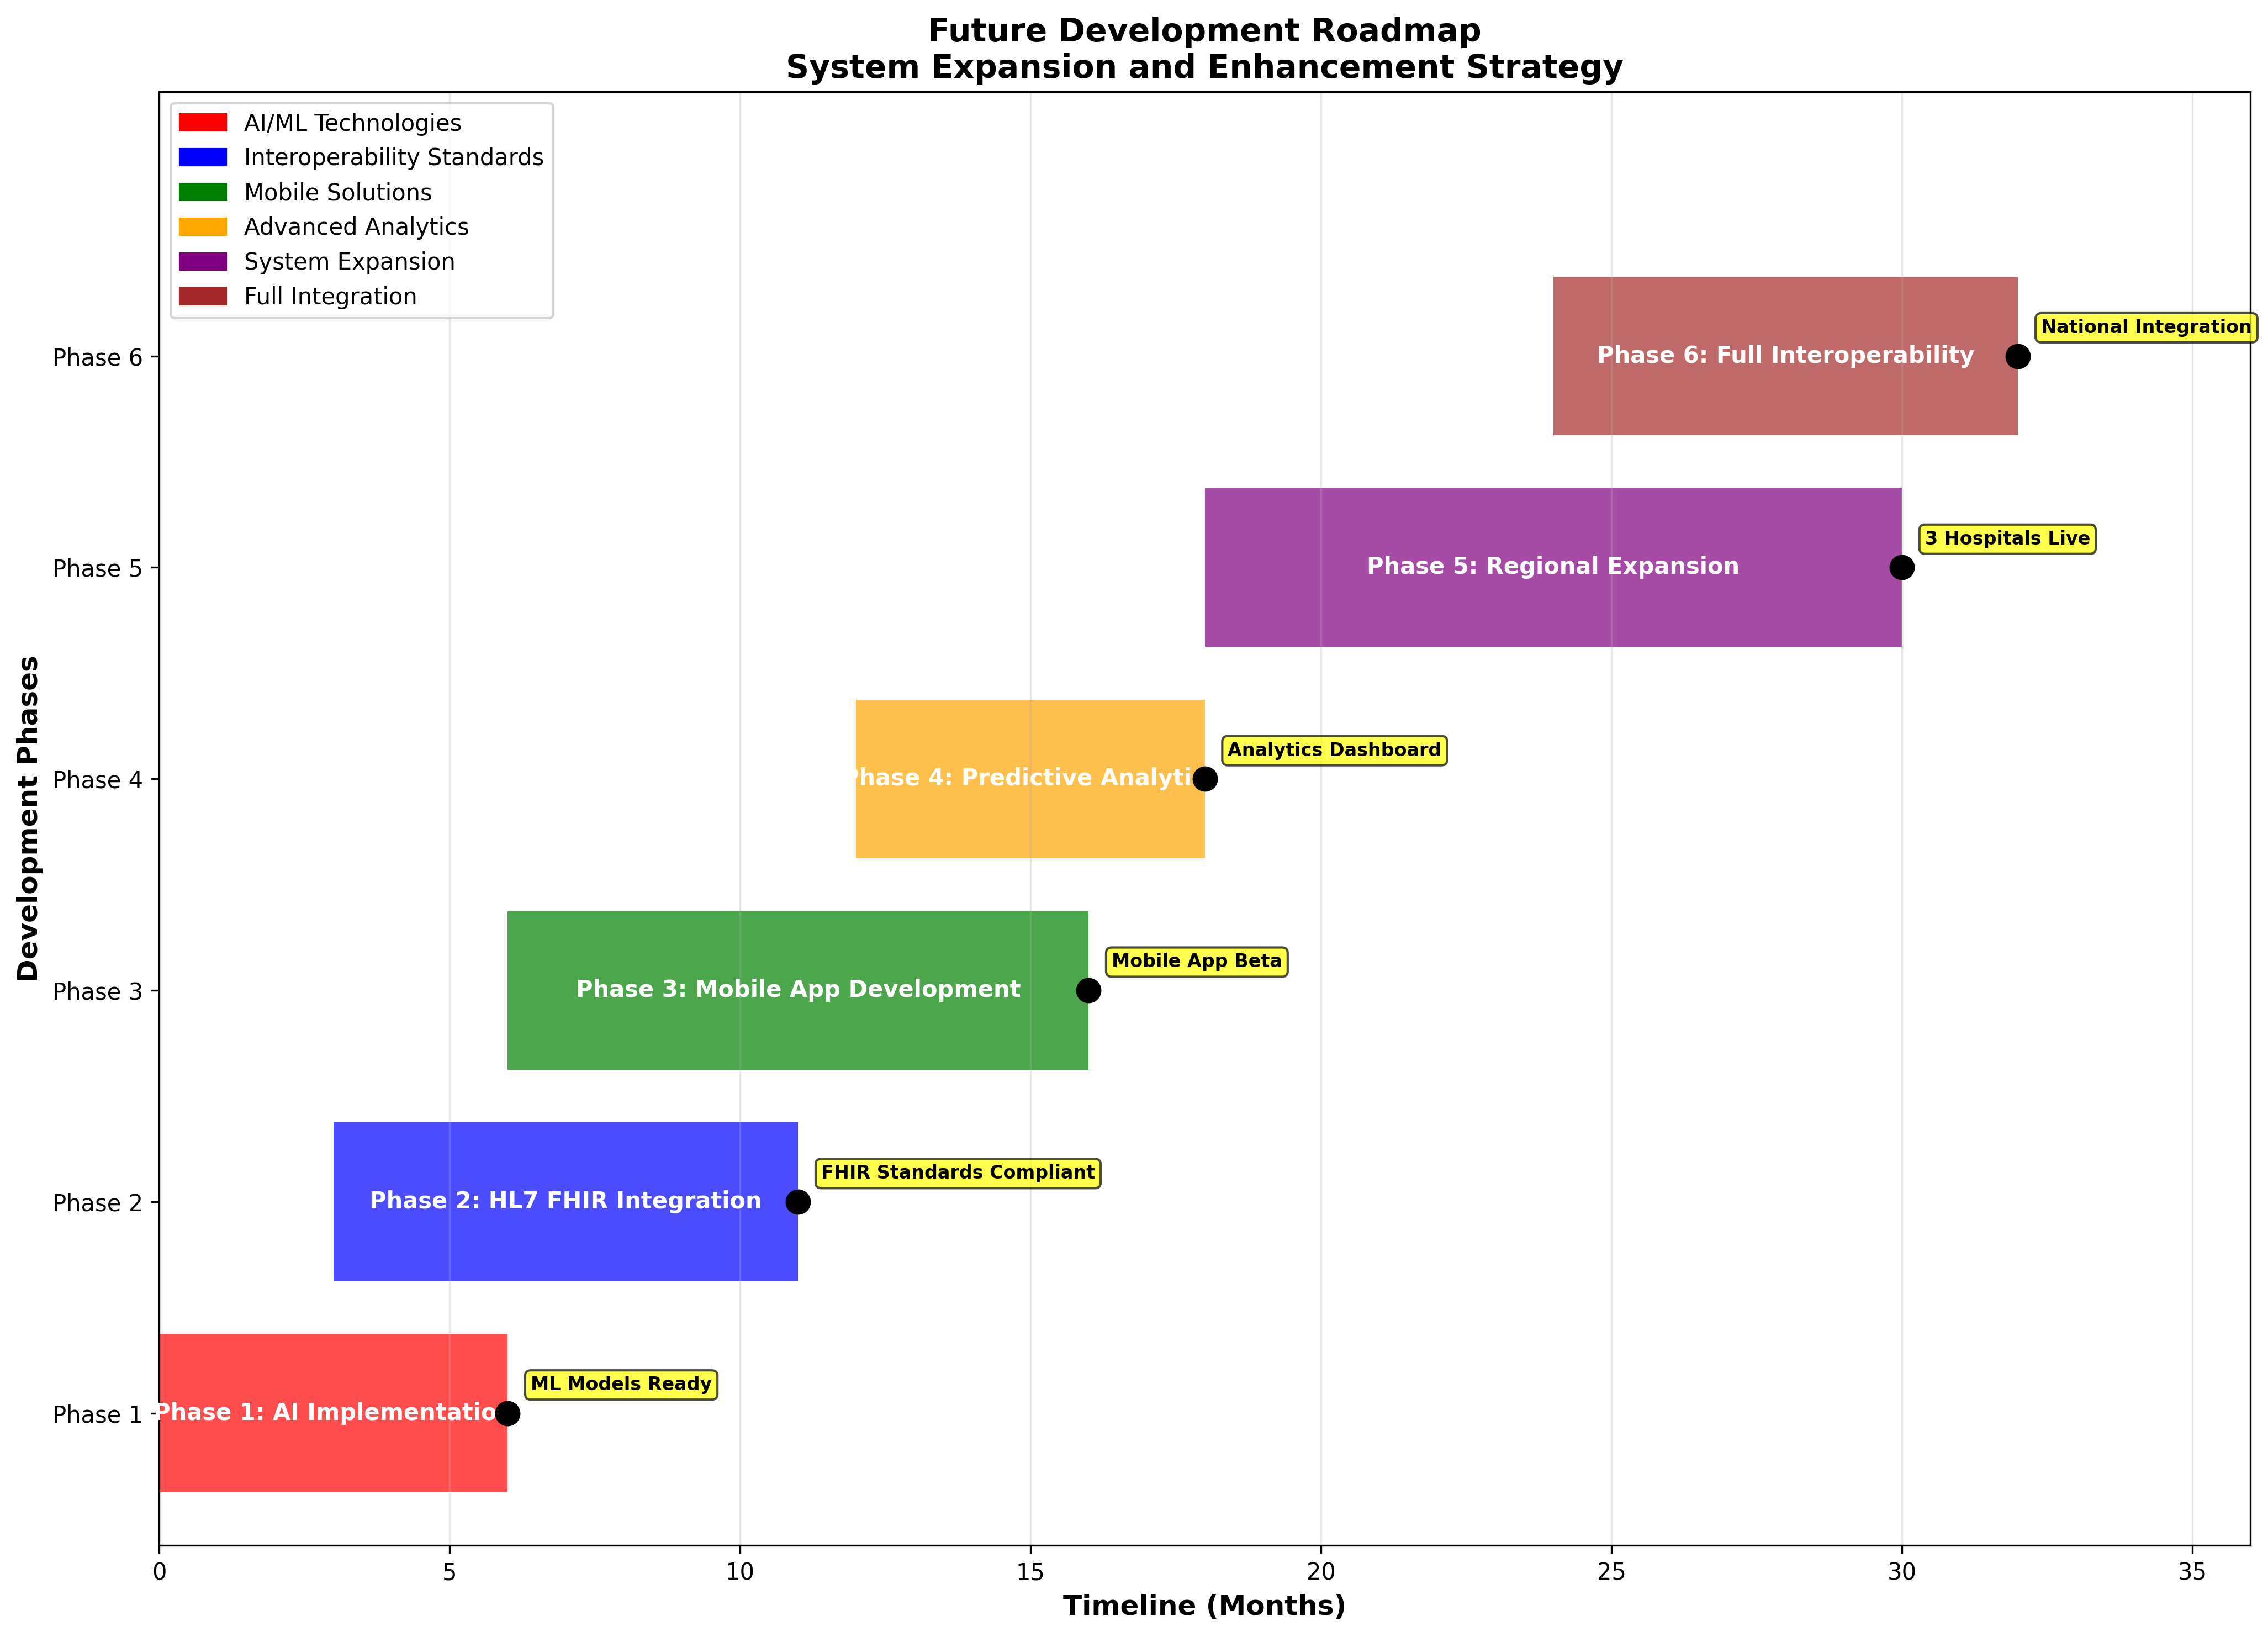
\includegraphics[width=0.95\textwidth]{images/generated/future_roadmap.png}
    \caption{18-month future development roadmap, including AI/ML features, FHIR integration, mobile application development, and regional expansion.}
    \label{fig:future-roadmap}
\end{figure}

\subsection{Key Performance Indicators and Evaluation Scenarios}
\label{sec:KPIs}

To anchor the evaluation in the concrete operational realities of SCMVV, the pilot study will focus on a set of specific Key Performance Indicators (KPIs), grounded in the real-world challenges described by the clinical staff. The following scenarios and metrics will be used to quantify the system's impact, contextualized by the broader issues of system fragmentation in the Portuguese NHS \cite{goiana2024portuguese, nunes2021articulacao}.

\subsubsection{Patient Safety and Clinical Quality}
The evaluation will primarily focus on the reduction in medication errors. This will be measured by comparing error rates (e.g., incorrect dosage, wrong medication, missed administrations) from a retrospective analysis of 1,000 prescriptions before the intervention with a prospective analysis of 1,000 prescriptions after implementation. A further metric will be adherence to protocols, assessed by auditing the system's logs to quantify the percentage of prescriptions that fully comply with the integrated clinical decision support rules.

\subsubsection{Operational Efficiency}
To measure gains in efficiency, the study will analyze time-in-motion for nursing staff. This involves observing and timing the end-to-end process of medication administration for a sample of 30 cases before and after implementation, from prescription verification to patient delivery. Additionally, the pharmaceutical validation time will be measured by calculating the average time from a physician's prescription entry to its final validation by a pharmacist in the system's backend, comparing the performance against the current multi-system workflow.

\subsubsection{System Integration and Data Integrity}
The success of the integration will be quantified by measuring the reduction in data redundancy and discrepancies. This will be achieved by performing a comparative analysis of patient records across the integrated systems (SClínico, AIDA, SONHO) before and after implementation, identifying and counting inconsistencies in key data fields (e.g., patient identifiers, active medication lists) to demonstrate a measurable improvement in data coherence, a known challenge in fragmented health information environments \cite{pinto2016identification}. 